\documentclass[a4paper]{article}

\usepackage[utf8]{inputenc}
\usepackage{fancyhdr}
\usepackage{float}
\usepackage{graphicx}
\usepackage{varioref}
\usepackage{url}
\usepackage[margin=1em]{subfig}
\usepackage{pgfplots}
\usepackage{tikz}
\usetikzlibrary{arrows}
\usetikzlibrary{positioning}
\pagestyle{fancy}
\graphicspath{{img/}}
\renewcommand\thepart{\Alph{part}}
\pgfplotsset{compat=1.5}

\newcommand\TODO[1]{\textcolor{red}{TODO:#1}}
\newcommand\todo[1]{\TODO{#1}}

\title{Homework Module: A Controller for Swarm Behaviour in Webots}

\lhead{Homework Module \#1}
\rhead{IT3708 - Subsymbolic Methods in AI}

\author{
    Aleksander Burkow \\
    Sigve Sebstian Farstad \\
    Emil Grønnbeck
}

\begin{document}
\pagenumbering{roman}

\maketitle
\thispagestyle{empty}

\abstract{
This report presents a solution for Homework Module \#1 of IT3708, spring 2014 at NTNU.
The purpose of the homework module is to ``understand swarm behaviour by implementing a controller for box pushing task in Webots''~\cite{assignment}.
}

\newpage

\tableofcontents

\newpage
\setcounter{page}{1}
\pagenumbering{arabic}

\part{Introduction}
\label{part:proposed-system}

``Swarm robotics is a field that capitalizes on self-organization to generate interesting global patterns from interactions among relatively simple robots, all in the absence of centralized control.''~\cite{course-page}

This report presents a homogenous robotic swarm that can identify interesting objects and push them to desired areas.
The individual agent is inspired by ant behaviour.



\section{Subsumption Architecture}
The implemented system is based on an AI concept called subsumption.
The subsumption architecture was first described by Rodney Brooks in 1986~\cite{brooks}, and is also called Brooks' Architecture.
The idea behind Brooks' Architecture is inspired by insect behaviour.
Insects, although they have relatively small amounts of computational power, are able to walk, avoid obstacles, and make complex decicions at impressive speeds.
The architecture is divided into behavioural layers called: "the levels of competence".\todo{cite where "the levels of competence" is from}.
Each layer is independent of the others, but the higher levels are capable of overriding the lower.~\cite{mwarnerwu}
This way, complex behaviour can be composed of many small reactive agent behaviours.

\section{Webots}

\section{The Epuck}

\begin{figure}[H]
\centering
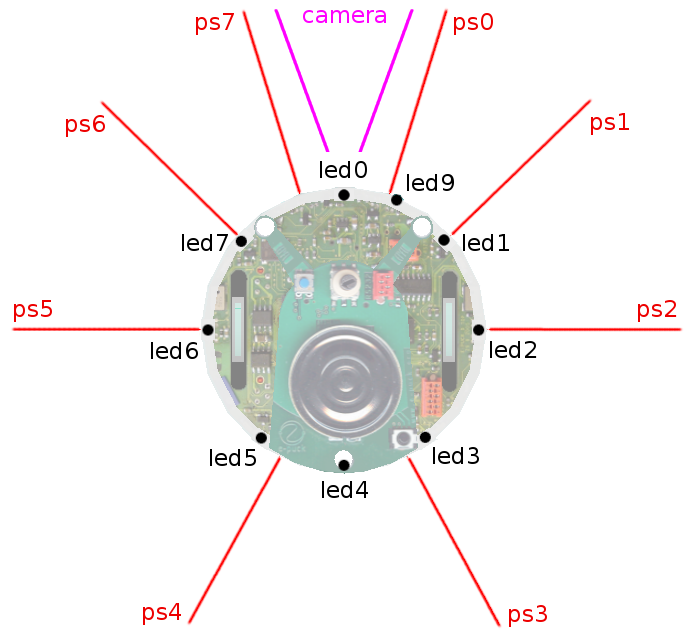
\includegraphics[scale=0.2]{e-puck_sensors_and_leds.png}
\caption{E-puck robot with all sensors}
\end{figure}

\part{The Proposed System}

\section{Description}

The initial proposed system is based on the subsumption approach suggested in \cite{assignment}.
The "levels of competence" are divided into six independent behaviours: Wander, Avoid obstacles, Converge, Retrieve, and Reposition.
The lower levels have a higher priority and are able to override the higher ones.
Figure \vref{figure:subsumption} shows the subsumption hierarchy.

\begin{figure}[H]
\centering
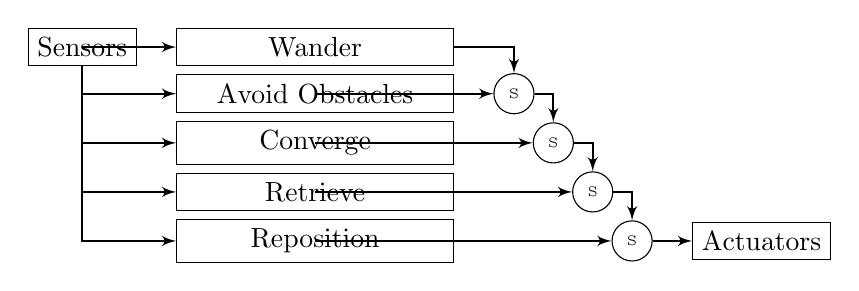
\begin{tikzpicture}

\tikzstyle{behaviour}=[draw, minimum width=10em, right=5mm of sensors]
\tikzstyle{line}=[draw, thick, -latex']
\tikzstyle{subsumption}=[draw, circle]

\node[draw] (sensors) {Sensors};

\node[behaviour] (wander) {Wander};
\node[behaviour, below=1mm of wander] (avoid_obstacles) {Avoid Obstacles};
\node[behaviour, below=1mm of avoid_obstacles] (converge) {Converge};
\node[behaviour, below=1mm of converge] (retrieve) {Retrieve};
\node[behaviour, below=1mm of retrieve] (reposition) {Reposition};

\node[subsumption, right=5mm of avoid_obstacles] (avoid_obstacles_subsumption) {\tiny S};
\node[subsumption, right=10mm of converge] (converge_subsumption) {\tiny S};
\node[subsumption, right=15mm of retrieve] (retrieve_subsumption) {\tiny S};
\node[subsumption, right=20mm of reposition] (reposition_subsumption) {\tiny S};
\node[draw, right=5mm of reposition_subsumption] (actuators) {Actuators};

\path[line] (sensors) |- (wander);
\path[line] (sensors) |- (avoid_obstacles);
\path[line] (sensors) |- (converge);
\path[line] (sensors) |- (retrieve);
\path[line] (sensors) |- (reposition);

\path[line] (avoid_obstacles) |- (avoid_obstacles_subsumption);
\path[line] (converge) |- (converge_subsumption);
\path[line] (retrieve) |- (retrieve_subsumption);
\path[line] (reposition) |- (reposition_subsumption);

\path[line] (wander) -| (avoid_obstacles_subsumption);
\path[line] (avoid_obstacles_subsumption) -| (converge_subsumption);
\path[line] (converge_subsumption) -| (retrieve_subsumption);
\path[line] (retrieve_subsumption) -| (reposition_subsumption);
\path[line] (reposition_subsumption) -- (actuators);

\end{tikzpicture}
\caption{The subsumption architecture of the proposed system.}
\label{figure:subsumption}
\end{figure}


\subsection{Behaviours}
Each of the behaviours of the proposed system are independent reactive behaviours that map input sensor data to output actuators. The rest of this section describes each of the behaviours in detail.

\subsubsection{Wander}
Wander is the default behaviour.
It tells the agent to move straight forward as fast as possible, regardless of input.

\subsubsection{Avoid obstacles}
This behaviour is intended to save the agent from harmful collisions.
It is triggered when the agent's proximity sensors rise above a certain threshold, indicating that it's close to or about to hit a wall.
The rotational angle of the agent is then set proportional to the difference between the amount of obstacles on either side of the agent.
The closer the wall is on the right side, the harder the agent will turn to the left, and vice versa.
This technique is called Braitenberg avoidance~\cite{braitenberg}.

\subsubsection{Converge}
This behaviour is intended to let agents converge on a food location.
It is triggered when the sum of the agent's light sensors rise above a certain threshold, indicating that food is nearby.
The rotational angle of the agent is set in proportion to the amount of light on either side, making the agent heads towards the food, aligning it with the surface normal of the food for maximum force.

\subsubsection{Retrieve}
This behaviour is intended to let agents push food to a goal area, and is triggered when the agent detects that food is right in front of it.
It will try to align the agent with the surface-normal of the object, such that maximum force will be exerted upon it.

It subsumes the obstacle avoidance behaviour, letting the agent push the food.

\subsubsection{Reposition}
This behaviour is intended to let agents to move out of potentially poor retrieval positions.
It is enabled when the agent has found food, and is trying to bring it home.

A problem that commonly occurs is that the agents are trying to push the food from opposing sides, and therefore getting nowhere.
The reposition behaviour simply says that after $ N $ seconds of retrieval, the agent will try to push somewhere else nearby.

This exponential backoff-inspired behaviour allows the agents to reposition themselves reasonably efficiently.

\section{Simulation Results}
\label{section:first-sim-results}

This version of the swarm agent was run in a series of simulation experiments in Webots.
7 swarm robots were randomly placed in a $ 1.5m \times 1.5m $ square world together with a randomly placed lit food block.
For each experiment, the time taken from world setup was complete until the swarm managed to transport the food to an edge of the world was measured.

This simulation was run 75 times.
The results of the simulation can be seen in figure \vref{figure:first-hist}.

\subsection{Observed weaknesses}

During observation of the 75 simulation runs, several weaknesses of the agent system were identified; amongst them: low levels of emergent teamwork, and getting stuck.

\subsubsection{No incentive for teamwork}
In the current architecture, the reposition behaviour blindly sends the robot away after it has been pushing the food for a fixed amount of time.

This does not entice teamwork, as robots who by chance are pushing on the same side have equal chance of repositioning themselves as robots who are blindly pushing from some unproductive angle.

This results in robots not intentionally clustering together, making food retrieval more luck-of-the-draw based than a coordinated operation.

\subsubsection{Getting stuck}
In this implementation, the robots have a tendency to get stuck in a few different ways:

\begin{itemize}
	\item Two robots driving straight into each other
	\item Getting stuck behind boxes
	\item Poor sensor calibration sometimes leads to robots not avoiding walls when food is nearby
	\item Rolling on their sides
\end{itemize}

\part{An Improved System}

\section{Description}

\section{Simulation Results}

This version of the swarm agent was run in a series of simulation experiments in Webots identical to the simulations in section \vref{section:first-sim-results}.

This simulation was run 75 times.
The results of the simulation can be seen in figure \vref{figure:second-hist}.

As hoped, the improved system presents a considerable improvement over the original system presented in part \vref{part:proposed-system}.
Indeed, the median completion time of the improved swarm agent is almost halved from the original agent, bringing it down to a somewhat impressive $ 21.344 $ seconds.

\part{A More Advanced Architecture}

\section{Description}
\section{Simulation Results}

\newsavebox{\zoomsinglegood}
\savebox{\zoomsinglegood}{%
\begin{tikzpicture}
\begin{axis}[
width=\textwidth/4,
ybar interval,
xtick=,% reset from ybar interval
yticklabel={\tiny $\pgfmathprintnumber\tick$},
xticklabel={\tiny $\pgfmathprintnumber\nexttick$},
]
\addplot+[hist={data={x}, bins=20, data max=250, intervals=false}]
file {measurements/1-box-7-epucks-without-unstick-random-placements-b35d4c771d6b71e88f73cf833ed8067aad97f4ff.txt};
\draw[red] (axis cs:21.344,0) -- (axis cs:21.344,18);
\end{axis}
\end{tikzpicture}
}

\newsavebox{\zoomsinglebad}
\savebox{\zoomsinglebad}{%
\begin{tikzpicture}
\begin{axis}[
width=\textwidth/4,
ybar interval,
xtick=,% reset from ybar interval
yticklabel={\tiny $\pgfmathprintnumber\tick$},
xticklabel={\tiny $\pgfmathprintnumber\nexttick$},
]
\addplot+[hist={data={x}, bins=20, data max=250, intervals=false}]
file {measurements/1-box-7-epucks-without-unstick-random-placement-bad-reposition-0c4ad0674e83c6681d4769371fe55f976d71ab72.txt};
\draw[red] (axis cs:38.336,0) -- (axis cs:38.336,18);
\end{axis}
\end{tikzpicture}
}


\begin{figure}[p]%
\centering
\subfloat[Randomly generated scenario with 1 food box and 7 epuck robots, with static reposition, without the unstick behaviour.]{{
\label{figure:first-hist}
\begin{tikzpicture}
\begin{axis}[
width=\textwidth/2,
ybar interval,
xlabel=Time to completion in seconds,
ylabel=Number of runs,
ymax=70,
xtick=,% reset from ybar interval
xticklabel={$\pgfmathprintnumber\nexttick$}
]
\addplot+[hist={data={x}, bins=20, data max=2000, intervals=false}]
file {measurements/1-box-7-epucks-without-unstick-random-placement-bad-reposition-0c4ad0674e83c6681d4769371fe55f976d71ab72.txt};
\draw[red] (axis cs:38.336,0) -- (axis cs:38.336,60) node [right=0.1cm] {38.336 s};
\draw (axis cs:1500,50) node {\usebox{\zoomsinglebad}};
\end{axis}
\end{tikzpicture}
}}%
\subfloat[Randomly generated scenario with 1 food box and 7 epuck robots without the unstick behaviour.]{{%

\begin{tikzpicture}%
\begin{axis}[
width=\textwidth/2,
ybar interval,
xlabel=Time to completion in seconds,
ylabel=Number of runs,
ymax=70,
xtick=,% reset from ybar interval
xticklabel={$\pgfmathprintnumber\nexttick$}
]
\addplot+[hist={data={x}, bins=20, data max=2000, intervals=false}]%
file {measurements/1-box-7-epucks-without-unstick-random-placements-b35d4c771d6b71e88f73cf833ed8067aad97f4ff.txt};%
\draw[red] (axis cs:21.344,0) -- (axis cs:21.344,60) node [right=0.15cm] {21.344 s};%
\draw (axis cs:1500,50) node {\usebox{\zoomsinglegood}};
\end{axis}%
\end{tikzpicture}%

}}%





\qquad
\subfloat[Randomly generated scenario with 2 food boxes and 7 epuck robots without the unstick behaviour.]{{
\begin{tikzpicture}
\begin{axis}[
width=\textwidth/2,
ybar interval,
ymax=70,
xlabel=Time to completion in seconds,
ylabel=Number of runs,
ymax=70,
xtick=,% reset from ybar interval
xticklabel={$\pgfmathprintnumber\nexttick$}
]
\addplot+[hist={data={x}, bins=20, data max=2000, intervals=false}]
file {measurements/2-boxes-7-epucks-without-unstick-random-placement-465bdfd2a08ceaf31540354378515dfb0287f40f.txt};
\draw[red] (axis cs:2000,0) -- (axis cs:2000,40) node [left] {Infinity};
\end{axis}
\end{tikzpicture}
}}%
\subfloat[Randomly generated scenario with 2 food box and 7 epuck robots with the unstick behaviour.]{{
\begin{tikzpicture}
\begin{axis}[
width=\textwidth/2,
ybar interval,
xlabel=Time to completion in seconds,
ylabel=Number of runs,
ymax=70,
xtick=,% reset from ybar interval
xticklabel={$\pgfmathprintnumber\nexttick$}
]
\addplot+[hist={data={x}, bins=20, data max=2000, intervals=false}]
file {measurements/2-boxes-7-epucks-with-unstick-random-placement-898fc092f762f5a17d5875ae62bb9baff5335149.txt};
\draw[red] (axis cs:647.872,0) -- (axis cs:647.872,20) node [right] {647.872 s};
\end{axis}
\end{tikzpicture}
}}%

\caption{Task completion measurement time distributions for different scenarios. Each scenario was simulated 75 times. The red line indicates the median time.
Smaller, embedded graphs are zoom-ins on specific ranges of the data set of the larger set.}
\label{figure:task-completion-times}
\end{figure}



\begin{figure}[H]
\centering
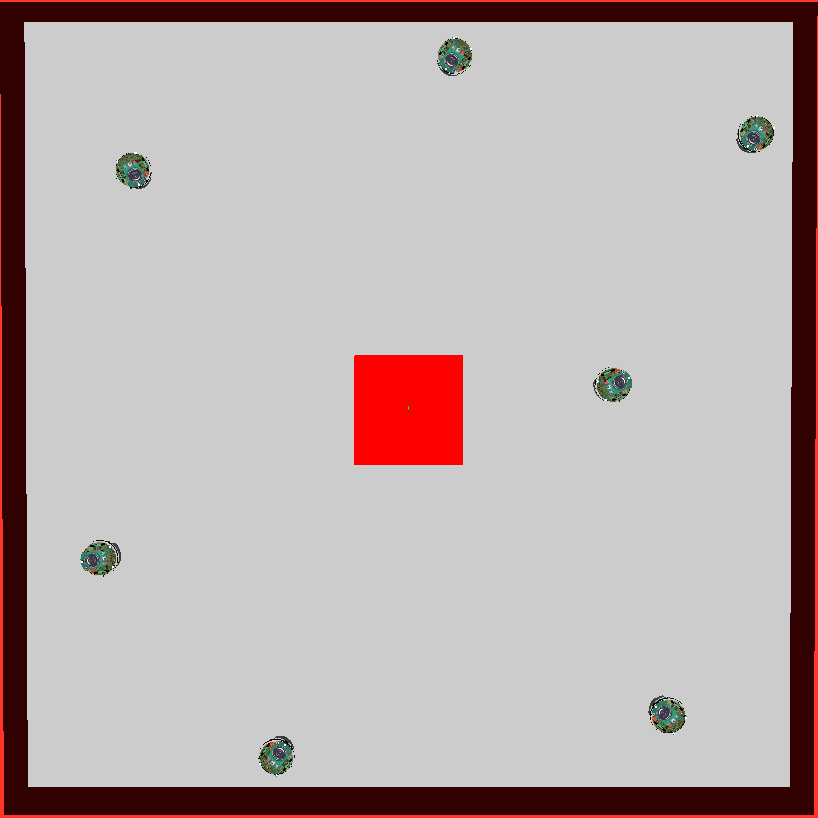
\includegraphics[scale=0.5]{one-box-world.png}
\caption{World used in the simulation for Table 1}
\end{figure}

\begin{figure}[H]
\centering
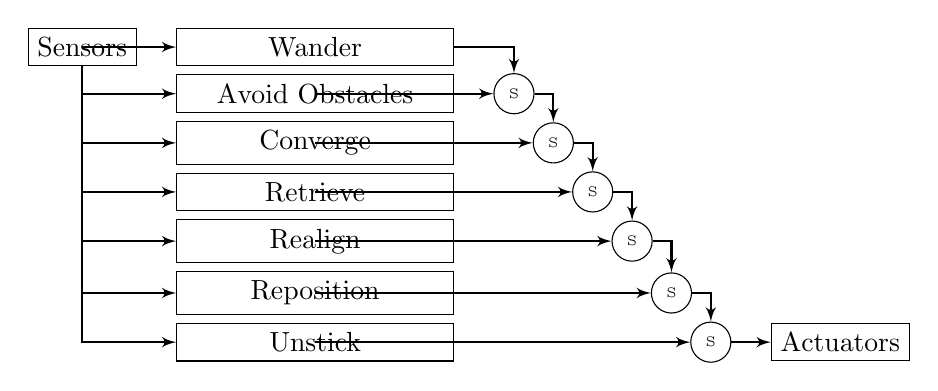
\begin{tikzpicture}

\tikzstyle{behaviour}=[draw, minimum width=10em, right=5mm of sensors]
\tikzstyle{line}=[draw, thick, -latex']
\tikzstyle{subsumption}=[draw, circle]

\node[draw] (sensors) {Sensors};

\node[behaviour] (wander) {Wander};
\node[behaviour, below=1mm of wander] (avoid_obstacles) {Avoid Obstacles};
\node[behaviour, below=1mm of avoid_obstacles] (converge) {Converge};
\node[behaviour, below=1mm of converge] (retrieve) {Retrieve};
\node[behaviour, below=1mm of retrieve] (realign) {Realign};
\node[behaviour, below=1mm of realign] (reposition) {Reposition};
\node[behaviour, below=1mm of reposition] (unstick) {Unstick};


\node[subsumption, right=5mm of avoid_obstacles] (avoid_obstacles_subsumption) {\tiny S};
\node[subsumption, right=10mm of converge] (converge_subsumption) {\tiny S};
\node[subsumption, right=15mm of retrieve] (retrieve_subsumption) {\tiny S};
\node[subsumption, right=20mm of realign] (realign_subsumption) {\tiny S};
\node[subsumption, right=25mm of reposition] (reposition_subsumption) {\tiny S};
\node[subsumption, right=30mm of unstick] (unstick_subsumption) {\tiny S};
\node[draw, right=5mm of unstick_subsumption] (actuators) {Actuators};

\path[line] (sensors) |- (wander);
\path[line] (sensors) |- (avoid_obstacles);
\path[line] (sensors) |- (converge);
\path[line] (sensors) |- (retrieve);
\path[line] (sensors) |- (realign);
\path[line] (sensors) |- (reposition);
\path[line] (sensors) |- (unstick);

\path[line] (avoid_obstacles) |- (avoid_obstacles_subsumption);
\path[line] (converge) |- (converge_subsumption);
\path[line] (retrieve) |- (retrieve_subsumption);
\path[line] (realign) |- (realign_subsumption);
\path[line] (reposition) |- (reposition_subsumption);
\path[line] (unstick) |- (unstick_subsumption);

\path[line] (wander) -| (avoid_obstacles_subsumption);
\path[line] (avoid_obstacles_subsumption) -| (converge_subsumption);
\path[line] (converge_subsumption) -| (retrieve_subsumption);
\path[line] (retrieve_subsumption) -| (realign_subsumption);
\path[line] (realign_subsumption) -| (reposition_subsumption);
\path[line] (reposition_subsumption) -| (unstick_subsumption);
\path[line] (unstick_subsumption) -- (actuators);

\end{tikzpicture}
\caption{The subsumption architecture of Bearded Octoninja.}
\label{figure:subsumption}
\end{figure}


\newpage
\pagenumbering{gobble}
\bibliography{reference-library}
\bibliographystyle{plain}

\end{document}
